\documentclass[twoside,11pt]{article}
/home/arya/workspace/projects/latex/macros-arya.tex
% Any additional packages needed should be included after jmlr2e.
% Note that jmlr2e.sty includes epsfig, amssymb, natbib and graphicx,
% and defines many common macros, such as 'proof' and 'example'.
%
% It also sets the bibliographystyle to plainnat; for more information on
% natbib citation styles, see the natbib documentation, a copy of which
% is archived at http://www.jmlr.org/format/natbib.pdf

\usepackage{jmlr2e}

% Definitions of handy macros can go here

%\newcommand{\dataset}{{\cal D}}
%\newcommand{\fracpartial}[2]{\frac{\partial #1}{\partial  #2}}

% Heading arguments are {volume}{year}{pages}{submitted}{published}{author-full-names}

\jmlrheading{}{}{}{}{}{}

% Short headings should be running head and authors last names

\ShortHeadings{}{}
\firstpageno{1}

\usepackage[linesnumbered,ruled]{algorithm2e}
\begin{document}

\title{DataRank: An Online Ranking Algorithm for Ranking Biomedical Datasets}

%\author{\name Arya Iranmehr, MS \email airanmehr@ucsd.edu \\
%       \addr Department of Electrical and Computer Engineering\\
%       \AND
%       \name Huan Wang, MS \email huanwng@ucsd.edu \\
%       \addr Department of Computer Science and Engineering\\
%       \AND
%       \name Xiaoqian Jiang, PhD \email x1jiang@ucsd.edu \\
%       \name Wei Wei, MS \email w2wei@ucsd.edu \\
%       \addr Division of Biomedical Informatics\\
%       University of California, San Diego\\
%       9500 Gilman Dr., La Jolla, CA 92037, USA
%       }

\editor{}

\maketitle
\begin{abstract} 
In this paper, we propose an online ranking algorithm, DataRank for ranking biomedical datasets that are used in the papers indexed in PubMed Central. DataRank takes the bipartite citation graph between datasets and articles and dataset features, i.e. MeSH terms, as input and rank datasets according to their relevance to the searching query as well as user feedbacks. DataRank constituted dataset features by aggregating MeSH terms from the connected papers in the bipartite graph. For each search query, DataRank first maps the "free text query" to a MeSHQuery and yield an \emph{offline} ranking of datasets for the MeSHQuery using a Bayesian approach which the likelihood is proportional to Jaccard index and prior is proportional to number of citations of that dataset. DataRank is also extended to a \emph{online} algorithm by incorporating user-feedbacks regarding ranking relevance. The online DataRank again takes an Bayesian approach  which uses offline DataRank as its prior and computes its likelihood by estimating the user rating for unknown values using collaborative filtering. A demo web search engine has been developed to rank more than 20,000 dataset that has been discovered in more than 1 million papers.
\end{abstract} 


\section{Introduction} \label{sec:introduction}
Over the past decades, a wide range of datasets including clinical, gnomic, imaging, behavioural, etc. is created in biomedical research, and there is no unified and systematic way for retrieving them. Although several repositories(e.g. DBGap, TCGA, GEO, etc.) has been established \cite{nih-repo}, unfortunately like many cases of big-data applications with a "diminishing return", retrieval of datasets is getting harder as the number of repositories and active datasets increases. In fact, the current indexing and searching system suffers from a number of problems, including
\begin{enumerate}[(I)]
	\item {\bf Indexing} of datasets rely on human resources, which is a costly and noisy precess. \label{item:indexing}
	\item {\bf Searching} between and within the repositories is not well developed, and user should know the dataset and repository prior to search.
	\item {\bf Integration} of the repositories is widely ignored and indexing, searching and maintenance of each repository is being done independently.
	\item {\bf Privacy}, only contain public datasets, which are only a small fraction of all the datasets is being generated. (Not sure, should check it out later)
	\item {\bf Ranking} of search results of each repository is being done naively based matching of the query to the dataset's limited metadata.
	\item {\bf Recommendation} is now is a part of most of modern information retrieval systems with large amount of users and items, but it has not been considered for datasets and research scientists. \label{item:recommendation}
\end{enumerate}

In this paper, we provide a solution for problems \eqref{item:indexing}-\eqref{item:recommendation}, respectively by
\begin{enumerate}[(i)]
	\item {\bf Crawling} the PMC articles for patterns and rules provided by NIH to discover datasets directly from papers. \label{item:crawiling}
	\item {\bf Integrating} all the discovered datasets into one unified repository. \label{item:integrating}
	\item {\bf Providing}, general information for both private and public datasets.
	\item {\bf Ranking} datasets using different informative features including MeSH, number of citations, etc.
	\item {\bf Recommendation} of other datasets beyond current search results to make related datasets even more discoverable. \label{item:recommendation-sol}
\end{enumerate}


\begin{figure}\label{fig:bipartite}
\centering

\includegraphics[scale=0.7]{bipartite.png}
\caption{A bipartite graph between $m$ datasets and $n$ papers with MeSH terms as their features. PID and DID are Paper ID and Dataset ID respectively where existence of an edge between a paper and a dataset implies that dataset is used in that paper.}
\end{figure}

It should be noted that the task of crawling and indexing datasets is a non-trivial and independent task to others, so the methods and techniques for implementing it are outside of the scope of this manuscript. Therefore, in the rest of this paper we mainly focus on developing efficient methods for \eqref{item:integrating}-\eqref{item:recommendation-sol} and for the crawling task we take an simple method as follows: 
By creating regular expressions for all the citation rules provided by NIH for each repository we discovered more than 20,000 datasets out of more than 1 million PMC full text articles and created a bipartite graph between dataset ids and paper ids. The  product of crawling process is actually a bipartite graph, though incomplete, between articles and datasets. In the rest of this paper we describe our methodology to process this bipartite graph, Figure \ref{fig:bipartite}.

The rest of this paper is organized as follows: in section \ref{sec:background} we first review existing methods for enhancing information retrieval systems and then in section \ref{sec:methodology} we present out methods for the aforementioned problems. We outline implementation remarks and experimental study in section \ref{sec:Experiments} and finally we make conclusions and state possible future works in section \ref{sec:conclusions}.



\section{Background} \label{sec:background}
Probably, information retrieval is the point when hypes about "Big Data" are came into realization, because as repositories of data are getting larger, effective information retrieval is getting much complicated. For example, in order to close the gaps between the largest information retrieval system in NIH, PubMeD, and the rate of growth of the repository, a number of techniques has been including
\begin{itemize}
\item relevance ranking \cite{ranking-medline}, where documents are ranked according to Term-Frequency Inverse-Document-Frequency (TF-IDF) relevance to the free-text query.
\item query expansion \cite{mesh-query}, which the (mappable) tokens in the query mapped to a MeSH term using Automatic Term Mapping (ATM) \cite{pubmed-atm} and query is augmented with a set of MeSH terms,
\item relevance feedback \cite{refmed}, where user feedbacks in previous ranking results are used to improve ranking results,
\item etc. \cite{pubmed-survey}
\end{itemize}
developed to enhance retrieval of articles. By default, PubMed uses a hybrid approach to process a free-text query \cite{pubmed-help} by expanding the query using Automatic Term Mapping (ATM) \cite{pubmed-atm} and sorts the results in a reverse chronological order based on the document TF-IDF relevance to the query.

However, in the machine learning community tools and learning algorithms for ranking objects has been well developed \cite{yahoo-rank-challange}. For example, given a labeled dataset, i.e. having the rankings for every document, RankSVM \citep{svm-rank-j} trains a nonlinear model to predicts future ranking based on training set. RefMed \cite{refmed} uses RankSVM to learn a model for each query by incorporating user feedbacks as "training dataset labels" into training process. Unfortunately, like other ranking algorithms, RankSVM only works well when enough labeled training samples (user feedbacks) are provided to the learning algorithm, which is very unlikely in real world situations, to expect a user to rate all the search results.

During past two decades a wide range of methods for creating recommender systems has been developed \cite{recommender-survey} to address the problem of unknwon user ratings for majority of results. For instance, collaborative filtering is a well-known algorithm for estimating user ratings for set of items based on their similarities to set of rated items \cite{cff-survey}.

Roughly speaking, Datarank implements, relevance ranking, query expansion and  relevance feedback using a Bayesian approach without requiring a training process.

\section{Methodology} \label{sec:methodology}
The DataRank algorithm is an online algorithm which updated its predictive model after receiving explicit and implicit feedbacks from users. Specifically, we resort to incorporate user feedbacks explicitly you giving an option to the user to rate the search results, and we interpret user clicks as implicit feedbacks. Therefore, for every new user, the algorithm works in an offline manner and after receiving user feedbacks it updates the model to present user specific rankings. In the following parts we first describe the features and then explain our DataRank model offline ranking and finally extend offline DataRank to online setting.

\subsection{Features}
In this paper we use the corresponding set of MeSH terms as features for each articles and use the bag-of-words representation for representing documents. More precisely, the corpus $n$ articles is represented by a $d \times n$ binary matrix, $M\in \{0,1\}^{d\times n}$. Similarly we define the matrix of $X\in \{0,1\}^{d\times m}$ for representing $m$ dataset via bag-of-words of MeSH terms, where $\bfx_i$ is the $i^{th}$ column of $X$, is $i^{th}$ document in the corpus. Also, for each dataset, the dataset  label $\bfy_i$, is the dataset identifier which is a categorical variable, i.e., $\bfy \in \{{1\cdots m}\}^m$, the bipartite graph is represented via the adjacency matrix $A\in \{0,1\}^{n\times m}$. Since we are considering binary features for both documents and datasets, the dataset features can be readily obtained from the document features and adjacency matrix:
\beq
X=\min( MA , 1)
\eeq
where $\min(\cdot)$ is a elementwise operator over its matrix argument.

\subsection{Offline Ranking}
For the problem of ranking we consider a probabilistic approach and propose a graphical model to specify dependencies between random variables in the model. Therefore, $\bfx, \bfy$ should henceforth be understood as realizations of the corresponding random variables.
We also introduce another random variable $\bfq$ for search queries over the same sample space as $\bfx$, i.e., MeSH terms which $\bfq \in\{0,1\}^{d}$.  Finally, $\bfc$ is an (observed) random variable which defines a prior over the labels $\bfy$.
The graphical model shown in Figure \ref{fig:pgm}-(a). It should be noted that, in any case variables $\bfx$ (dataset features) and $\bfc$ (datasets prior) are observed and we never need their marginal distributions and therefore we only consider the query $\bfq$ as evidence.

In this model, the problems of ranking for a given query $\bfq$ is to find the posterior distribution for the dataset labels given evidence. More precisely the posterior distribution
\beq
\pr(\bfy | \bfq,\bfc, \bfx) \propto \pr(\bfy | \bfc ) \pr(\bfq | \bfx)
\eeq
full specifies the ranking, where the posterior distribution is expanded according to the graphical model Figure \ref{fig:pgm}-(a). 
Since, $\pr(\bfy | \bfc )$  is not function of evidence, we can legitimately consider it as dataset-prior and consider $\pr(\bfq | X)$ as query-likelihood.

In the standard statistical modelling procedures, the next step is to specify dataset-prior and query-likelihood distributions.

\paragraph{Query-likelihood.} Since the binary feature vector $\bfx$ and query $\bfq$ are representation of sets, using Vann diagram, we can easily compute the likelihood
\beq
\pr(\bfq | \bfx)= \frac{\pr(\bfq , \bfx)}{\pr(\bfx)} = \frac{|\bfq \cap \bfx|}{|\bfx|}
\eeq
where set operations are applied to the set representation of the binary vectors.

However, this probability does not account for mismatches in partial matching of terms in the query and features of each dataset, and this leads to the phenomena that two queries whit the same number of matches but different number of mismatches have the same probability. To remedy this crucial problem, we can add the number of mismatches to the denominator, which is equivalent to condition on $\bfx \cup \bfq$
\beq \label{eq:jaccard}
\widehat{\pr}(\bfq | \bfx ) \propto \pr(\bfq | \bfx \cup \bfq)= \frac{|\bfq \cap \bfx|}{|\bfq \cup \bfx|}
\eeq
the value of \eqref{eq:jaccard} is known as Jaccard index or Tanimoto or Jaccard coefficient \cite{book:IR}. Thus for the query likelihood we have
\beq \label{eq:jaccard}
\pr(\bfq | \bfx ) = \frac{\widehat{\pr}(\bfq | \bfx ) }{\sum_{i=1}^n \widehat{\pr}(\bfq | \bfx_i ) }
\eeq

\paragraph{Dataset-prior.} Instead of learning a prior for datasets using empirical Bayesian methods, we simply chose to propose a reasonable subjective prior for the datasets. Basically, the better way to think about prior is to imagine the posterior distribution in a scenario where there is no evidence available, which is equivalent to say that what is the best ranking of datasets if do not have a query. There are many ways to answer this question, but a reasonable approach is to sort them based on their general popularity. Interestingly, we can quantitatively specify the popularity for the datasets by taking into account of how many citations they have in the training dataset, i.e., $\bfc=\bfone^TA$. More precisely, we can write prior as
\beq \label{eq:prior}
\pr(\bfy | \bfc ) = \frac{\bfc}{ \bfc^T \bfone} = \frac{\bfone^TA}{\bfone^TA \bfone}
\eeq
where $\bfone$ is the vector of ones of corresponding dimension.
\begin{figure}
\centering
\begin{tabular}{cc}
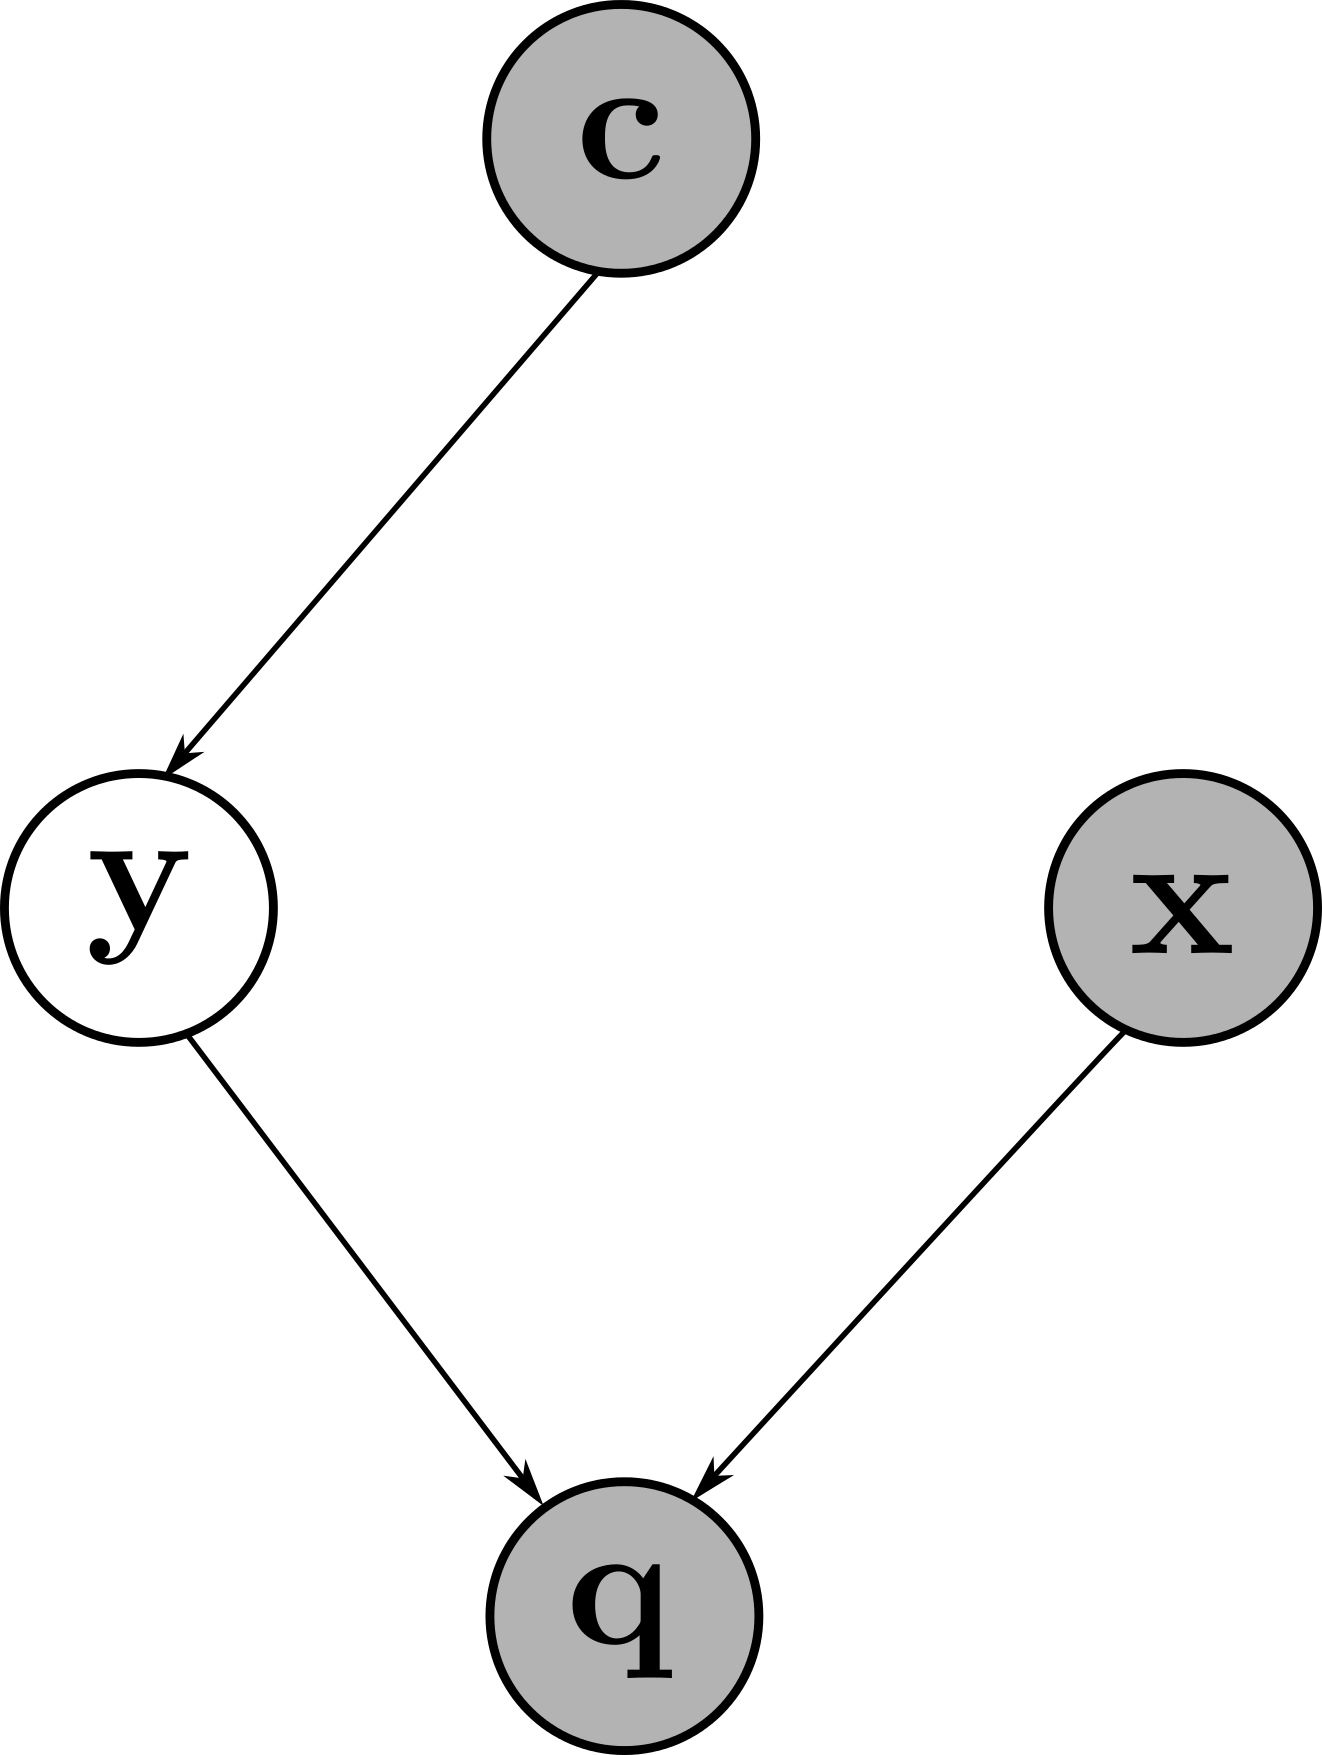
\includegraphics[scale=0.7]{offline-pgm.png} \hspace{0.3in} & 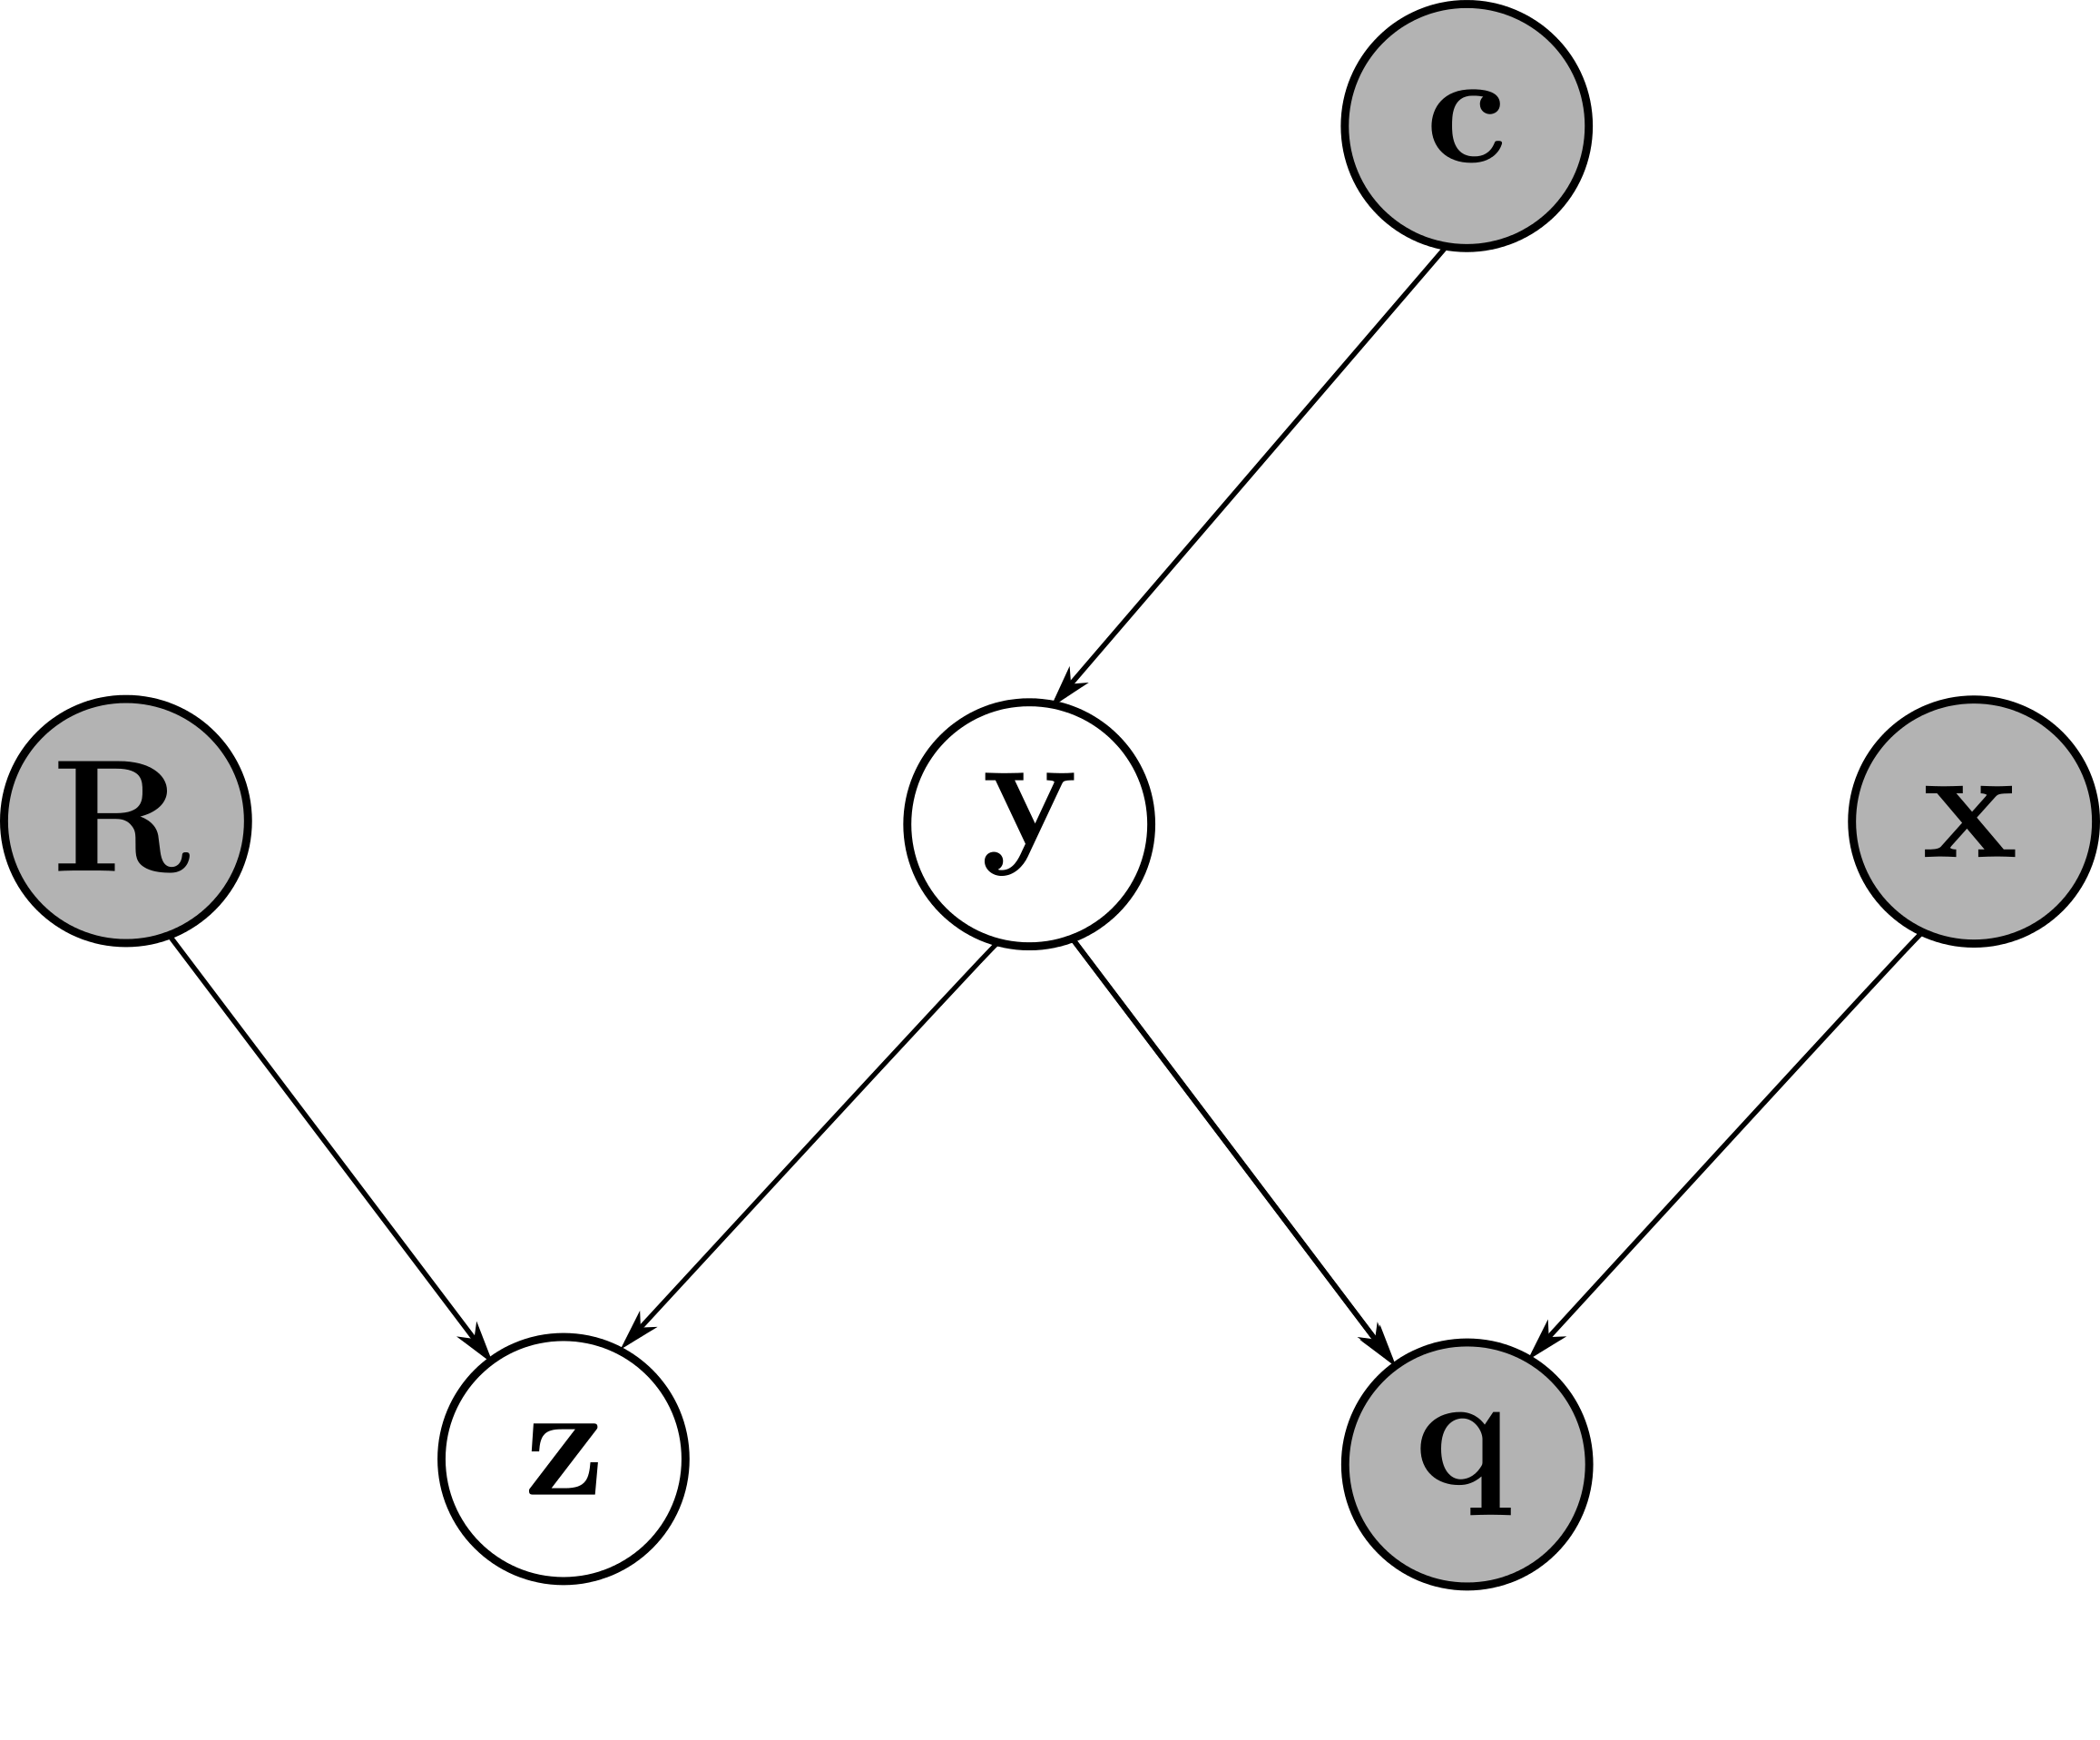
\includegraphics[scale=0.7]{online-pgm.png}\\
(a) & (b)
\end{tabular}
\caption{Probabilistic graphical models for offline (a) and online (b) methods for ranking datasets. The shaded nodes are observed variable, arrow implies conditional dependence and rectangles are short hand for replication of the inside nodes. For details see text.}\label{fig:pgm}
\end{figure}
So far, we have fully specified the prior and likelihood and hence posterior for the offline model and the ranking of datasets amounts to merely sort datasets decreasingly according to their posterior distribution.
\subsection{Online Ranking}
In this part we extend the offline-DataRank to the online setting by incorporating user feedback into ranking. For this porous, we propose a new model, Figure \ref{fig:pgm}-(b), which introduces \emph{incomplete} user ratings $\bfr\in \{0\cdots k \}^{m}$, and the dataset online-labels $\bfz$, where $k$ is the number of different state of ratings for each result in the ranking and 0 is used to denote unknown values in the ratings. Thus, in the ranking process, ratings $\bfr$ are initialized with zero value and at each epoch users rates the search results and updates the $\bfr_t$. As shown in the graphical model, the online-labels depend on user feedback but, (offline) dataset labels $\bfy$ do not. 

 Similar to offline method, the task is to compute the posterior
\beq \label{eq:online-posterior}
\pr (\bfz | \bfr, \bfy, \bfc, \bfq, \bfx)  \propto  \pr (\bfz |\bfr) \pr (\bfy |\bfc,\bfq, \bfx)
\eeq
where the factorization induced by the graphical model Figure \ref{fig:pgm}-(b) and in this model evidence is incomplete user rating $\bfr$. Interestingly the offline posterior $\pr (\bfy |\bfc,\bfq, \bfx)$ can be regarded as prior in this model, which implies that without any evidence, user ratings, the online posterior is exactly equal to its prior, i.e., offline posterior, which makes a perfect sense.

However, the ratings $\bfr$ is incomplete, i.e. contain zero values, and in order to specify the likelihood $\pr (\bfz |\bfr)$ we first need to estimate the unknown values of user ratings. Once we estimate all the unknown values in the user rating vector $\bfr$  we can readily  compute the likelihood $\pr (\bfz |\bfr)$ by normalizing $\bfr$

We use collaborative filtering \cite{CF-survey} to estimate unknown values of user ratings for the datasets that has not been rated yet. Collaborative filtering methods generally work by constructing a similarity matrix between items (dataset), and defining a method for finding a set of neighbours of each item, and then computes the rating of undated items as weighted linear combination its rated neighbours, where the weights are proportional to similarity between items.

Since the rating vectors is extremely sparse we choose to define the method for finding neighbours to return all the rated items, to use all the user rating information. Thus, the key step remains to perform collaborative filtering is to define a similarity measure between datasets. Regarding, the binary MeSH representation of datasets, we opt to use Tanimoto kernel \cite{t-kernel} between datasets for measuring similarity between datasets
\beq
K_{i,j} = K(\bfx_i,\bfx_j) =  \frac{\bfk_\cap(\bfx_i,\bfx_j)}{\bfk_\cap(\bfx_i,\bfx_i) + \bfk_\cap(\bfx_j,\bfx_j) - \bfk_\cap(\bfx_i,\bfx_j)}
\eeq
where $K$ is a $m \times m$ symmetric positive definite matrix, $\bfk_\cap(\bfx_i,\bfx_j)=\frac{|\phi(\bfx_i) \cap \phi(\bfx_j) |}{|\phi(\bfx_i) \cup \phi(\bfx_j)| }$ is intersection kernel \cite{i-kernel} between $\bfx_i$ and $\bfx_j$, and $\phi(\cdot)$ is a general nonlinear feature function. 

Having a similarity matrix between datasets, using collaborative filtering we can readily fill the unknown values in the completed rating vector $\bfR$ 
\beq
\bfR_i= 
\begin{cases} 
\bfr_i,  &\bfr_i \neq 0  \\
\bfr^TK_i , &\bfr_i = 0 \end{cases} 
\eeq
where $K_i$ is the $i^{th}$ column of the kernel matrix. Having computed the completed rating vector, to compute the likelihood, we only need to normalize $\bfR$
\beq \label{eq:online-likelihood}
\pr(\bfz | \bfr) = \frac{\bfR}{\bfone^T \bfR}
\eeq
Using \eqref{eq:jaccard} and \eqref{eq:online-likelihood} we can fully specify the online prediction posterior \eqref{eq:online-posterior} and therefore, online ranking for the DataRank algorithm.

\section{Experimental Study} \label{sec:Experiments}
\subsection{Implementation}
DataEngine is deployed on an Ubuntu 13.04 system with Intel Xeon X5650 2.67GHz and 4 GB RAM. Nginx 1.4.6 is used for static request and django 1.7.4 is used for dynamic request. uwsgi is used as an application server hosting django models, which is also used as an interconnector between nginx and django. Nginx is chosen for a consideration of future high traffic. A django/python combination is more extensible for future recommendation algorithm research with assistance of numpy and scipy.

%    \begin{figure}[htbp]
%        \centering
%        \includegraphics[width=0.95\linewidth]{imgs/Components.png}
%        \caption{Components Relation}
%        \label{fig:components_relation}
%    \end{figure}

    \subsubsection{System Architecture} % (fold)
    \label{ssub:system_architecture}
        A brief system architecture is shown below. The abstract architecture is a standard MVC model.
    
         \begin{figure}[htbp]
             \centering
             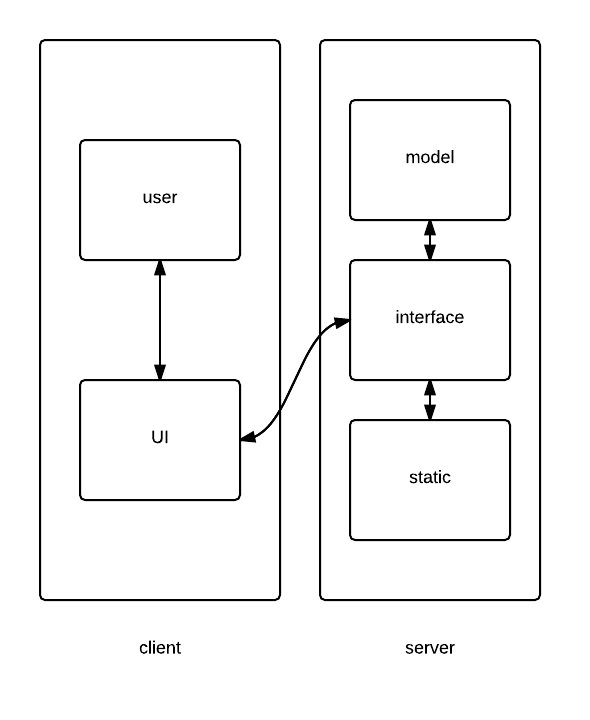
\includegraphics[width=0.95\linewidth]{architecture.png}
             \caption{System Components}
             \label{fig:system_components}
         \end{figure}

        All user interaction with UI is passed to interface layer for futuer response. All static request is passed to nginx and will be responsed immediately. Dynamic request is passed to model layer. After processing and computation, a response will be given back to user via same path.

        \begin{figure}[htbp]
            \centering
            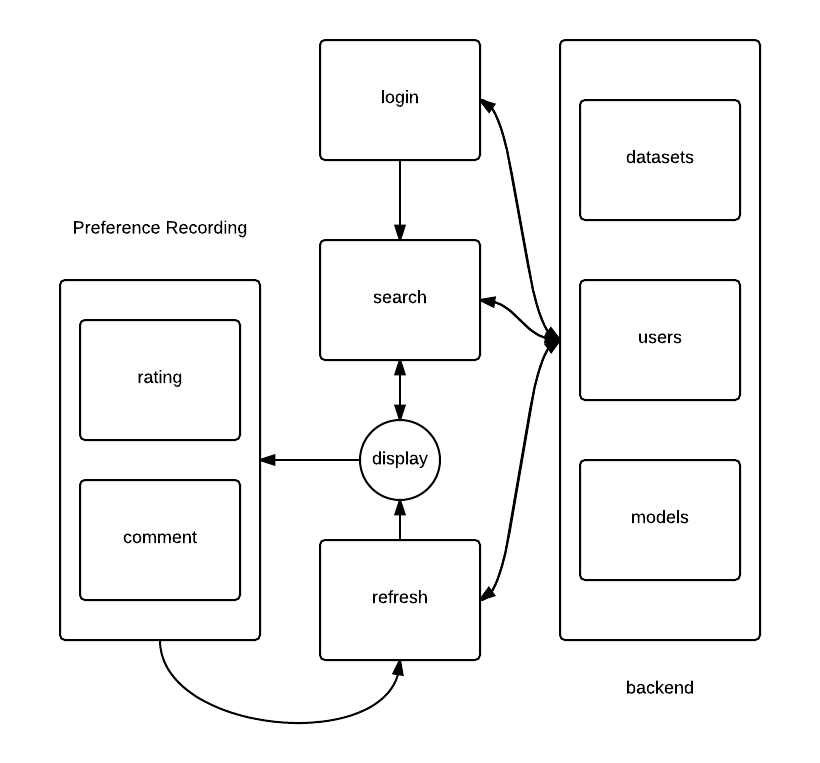
\includegraphics[width=0.95\linewidth]{workflow.png}
            \caption{}
            \label{fig:Work Flow}
        \end{figure}

        At system entry, there is a login management component. User could register, login or stay anonymous. When user either registered or logined, this user will be given a unique identifier. For identified user, all history action could be retrieved for recommendation and all new actions will be recorded as preferences. A search component works at next step. User insert one or a combination of keywords, a list of datasets will be shown on display via an offline ranking algorithm. Keywords will be passed to backend and be processed by a set of function and algorithms, and then a list of datasets is given with a keywords related order. The algorithm will be introduced on section \ref{sec:algorithm}.

        Display component plays as an important connector among different models and functions. User gives rates and comments on this step. When new user related information is added, a refresh component is activated. It will pass all new infomation to backend, and a backend online learning algorithm will collect all user historic and current preferrences and then give a new ranking based on updated information. This infomation will be shown on display component.

    % subsubsection system_architecture (end)

    \subsubsection{Searching Pattern} % (fold)
    \label{ssub:searching_pattern}

        Searching bar is the first function component faced by user. It could support several basic pattern. Current preffered keywords are MeSH terms. However there are punctuations included in existing MeSH terms text. We choose semicolon as splitter. When a string of keywords is passed to backend component, a grammar parser component is activated. it first changes keywords to lower letters, splits keywords by semicolons, and then remove travial characters for each keyword. A set of cleaned keywords will be passed to next model for further processing.

        Now, dataset specific searching is supported. User may have a destination data source. Thus supporting a data resource fixed searching pattern is necessary. We use an at sign (@) on the end of keywords, and dataset name is given after it. This dataset name is stored, and all future refreshing will only occur under this scale. A simple example is (DNA;Genes@GeneBank).

    % subsubsection searching_pattern (end)

    \subsubsection{Refresh} % (fold)
    \label{ssub:efresh}

        Refreshing is one of the most important feature in this system. Refreshing is majorly session based. A session is define as the a period of actions with one fixed query. If a new query is requested, a new session will be created. In a session, user could give ratings and update preferences unlimitedly. Everytime, when new information is given, an update of recommendation would be activated. A standard session work flow is: a user input keywords, and a list of datasets are given. After considering, user gives ratings to some of them and trigger refresh component. Relearning user preferences will be executed and a list of new ordered data will be given.
    
    % subsubsection refresh (end)

    \subsubsection{Ratings and Comments} % (fold)
    \label{ssub:ratings_and_comments}
        
        Ratings and comments are two important feature for online learning, which is introduced on section \ref{sec:algorithm}. As users may change their ideas frequently, ratings are stored on browser session, which provide better security than traditional cookies. Those ratings will be passed to server side and stored when refresh action is triggered. Each rating is a pair of dataset ID and rating score. Comments are also passed to server side with dataset id, and user related information will be added later. All stored ratings and comments include time information and user information and even keywords. All this information could be used for future ranking algorithm development.

    % subsubsection ratings_and_comments (end)

    \subsubsection{Assistant Information} % (fold)
    \label{ssub:assistant_information}
    
        In order to help user evaluate and understanding datasets orders better, we offer several parameters, such as posterior likelihood value (online ranking results) and raw prior probability. Counts of citations are also provided. All these statistics could be used as an compliment of metadata in order to have a better understanding of datasets.
\subsection{Experiments}
Unfortunately for such a novel problem, to this time, there is no labaled dataset which ground truth ranking of datasets are known. The lack of labeled dataset is not only a challenge for learning a predictive model, but also makes evaluation of the model more tricky. Yet, we set to perform two set of experiments to show that
\begin{enumerate}
\item by getting user feedbacks, DataRank actually learns about user preferences  
\item DataRank provides user-specialized results for each user
\end{enumerate}

In the first set of experiment we aim to show how well DataRank predicts user ratings, by comparing DataRank by gold-standard  ranking, the ranking in which is presented by DataRank given current features and actual user ratings, i.e. the best possible ranking using DataRank and full labels \cite{Shalev-shwartz2008}. 
Since the ranking is linearly related to its user rating, we measure the discrepancy between DataRank ranking and gold-standard DataRank rankings by just measure the \emph{loss} between the predicted value of rating and and the actual user rating. For instance, suppose at $t^{th}$ step user rates $j^{th}$ dataset, we can easily compute the loss
\beq
\bfl^{(t)}=|\hat{\bfr}_j^{(t-1)} -\bfr_j^{(t)}|
\eeq
where $\hat{\bfr}$ is the predicted user rating in previous step.
Since the loss is quite instantaneous we smooth it by defining \emph{regret} \cite{Shalev-shwartz2008} as average loss until know
\beq
\bfR^{(t)}=\frac{1}{t} \sum_k^{t} |\hat{\bfr}_j^{(k-1)} -\bfr_j^{(k)}|
\eeq

we computed regret for each time for 5 different subjects and the rults for 20 feedbacks are shown in Figure \ref{fig:regret}.
It can be seen that regret has a global decreasing meaning that throughout time, DataRank make more accurate predictions.

For the second set of experiments we set different subjects search for the same query and rate the results according to their preferences. Then we  in this experiment we show that DataRank is able to present user special results. For this case user A and B search for the same query, e.g. "Mice", and $t=1\cdots T$ we compute the \emph{Kappa statistic} \cite{kappa} for measuring disagreement between users. For example we cam compute the ratings between users $A$ and $B$ at each time
\beq
\kappa_{A,B}^{(t)}=\kappa(\bfr_A^{(t)} , \bfr_B^{(t)})
\eeq
We again run this experiment for 5 subjects using the same query and computed parwise kappa score for all the users and depicted their average throughout time in Figure \ref{fig:dis}. Figure \ref{fig:dis} shows that even for the same query users tend to have disagreement which leads to different rating for each user.


\begin{figure}
\centering
\begin{tabular}{cc}
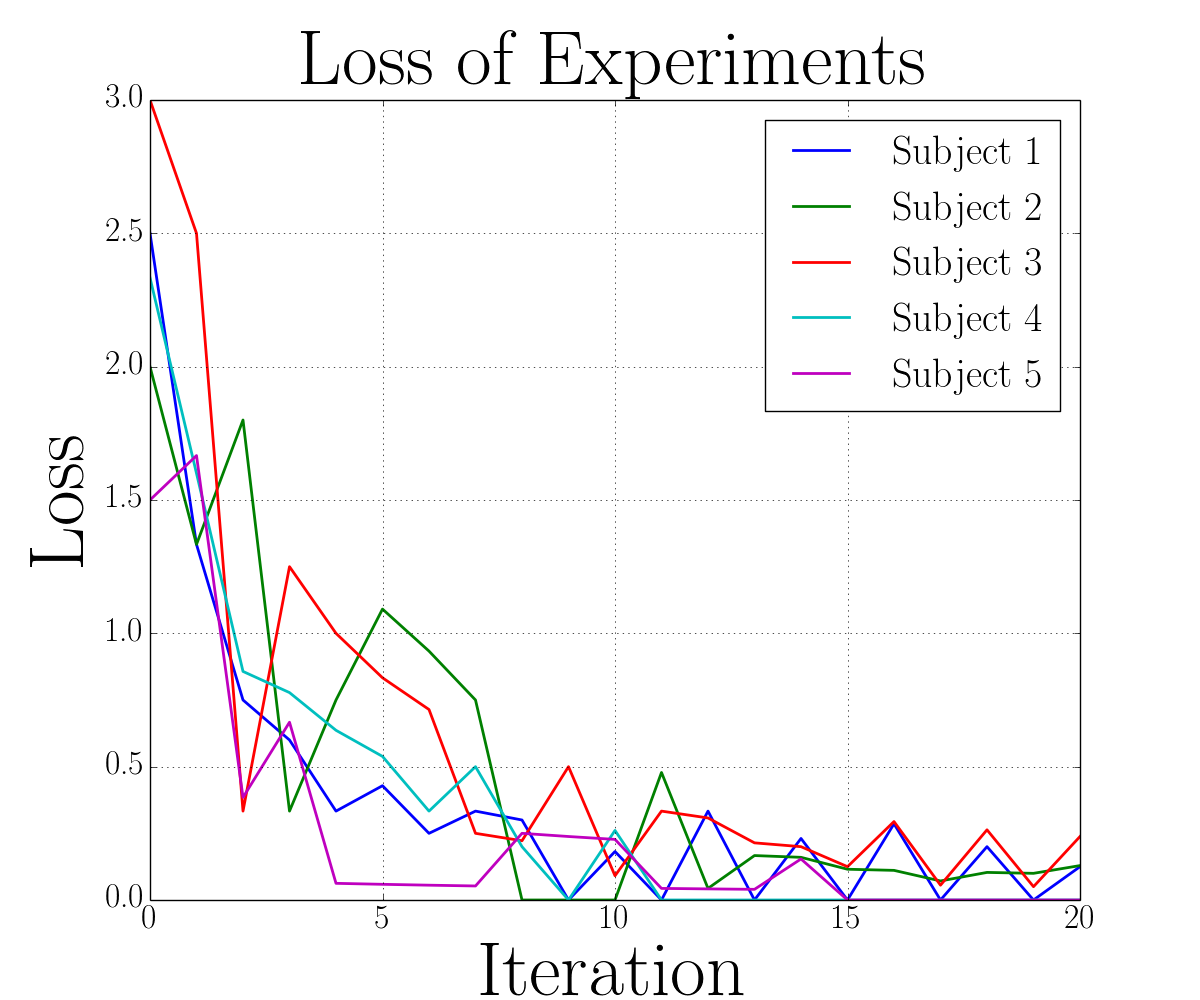
\includegraphics[scale=0.25]{Loss.png}  & 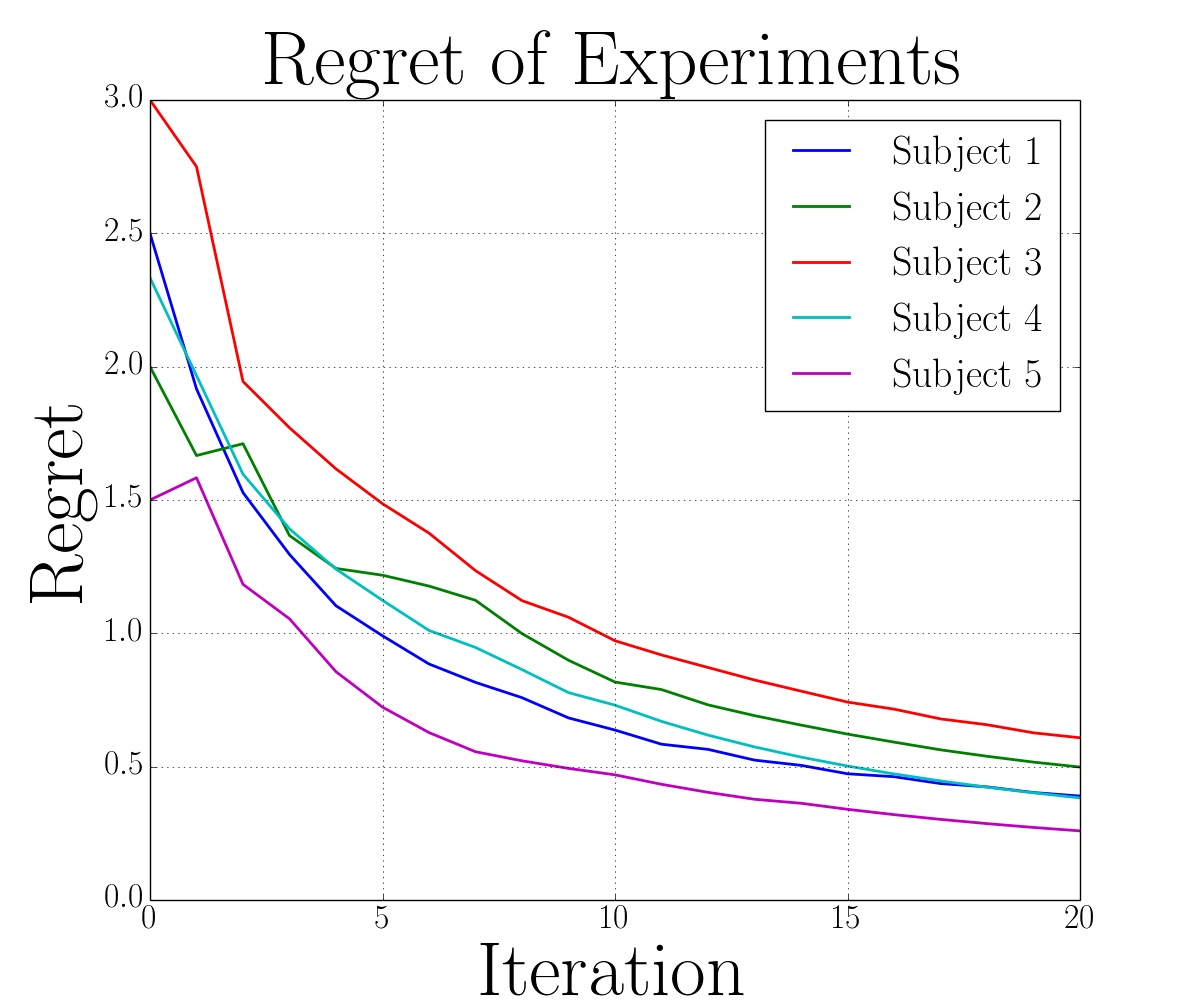
\includegraphics[scale=0.25]{Regret.png}\\
(a) & (b)
\end{tabular}
\caption{Loss and Regret of predicted ratings throoughout time.}\label{fig:regret}
\end{figure}

\begin{figure}
\centering
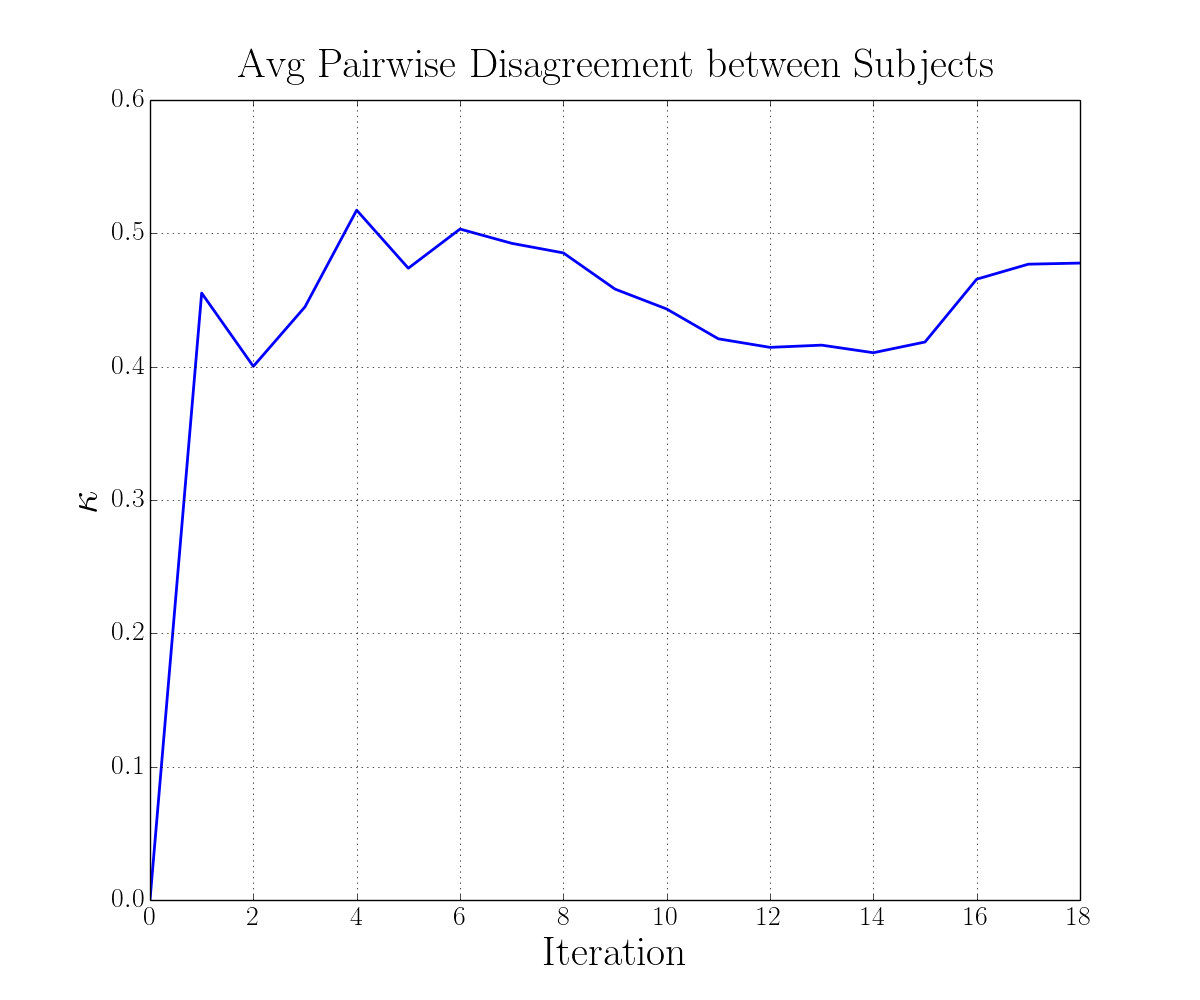
\includegraphics[scale=0.5]{dis.png} 
\caption{Average disagreement between users.}\label{fig:dis}

\end{figure}
\section{Conclusions} \label{sec:conclusions}
(Xiaoqian)

\bibliography{/home/arya/Documents/library}

\end{document}
